% Provenance (never printed): see sources/outline_sources.md (Year 2: mid-latitude cyclones and
% fronts; jets and Rossby waves, descriptive; tropical cyclones; numerical weather prediction,
% principle). Definitions after the NWS glossary and UCAR; cyclogenesis conditions after the NOAA
% AOML FAQ; potential intensity after Gilford (2021, pyPI); conveyor belts after Raveh-Rubin and
% Catto (2019); blocking after Wang and others (2026); predictability after Krishnamurthy (2019),
% Selz and others (2022) and ECMWF. The Lorenz system from figdata/bachelor-2/weather.py; the
% fronts, waves and storms of the examples, exercises and problem are invented, their values
% computed in the Book 4 scratch calculator calc/ch22.py.
\chapter{Sistemas meteorológicos}\label{ch:b2:weather-systems}

Uma previsão a quatro dias é hoje tão precisa quanto era, há trinta anos, uma previsão a um dia,
e cada década acrescentou cerca de um dia de previsão útil. No entanto, nenhuma previsão do
tempo de um dado dia, num dado lugar, é confiável muito além de dez dias, e computadores melhores
não bastarão para empurrar muito esse limite: a atmosfera amplifica suas próprias pequenas incertezas. Este
capítulo descreve os sistemas meteorológicos que as previsões acompanham, as frentes e as depressões das
latitudes médias, as ondas da corrente de jato e os ciclones tropicais, e depois a maneira como são
previstos e por que a previsão tem de parar em algum ponto.
% ledger: mo:accuracy, bauer:day-per-decade, krish19:predictability

\begin{recall}
\textbf{Dos volumes escolares}: massas de ar, frentes, frentes frias e quentes, depressões e
anticiclones, isóbaras e previsões do tempo; o ciclone tropical, seu olho e sua parede do olho, a
escala de Saffir--Simpson. \textbf{Do volume do primeiro ano}: a força do gradiente de pressão, o
parâmetro de Coriolis $f = 2\Omega\sin\varphi$, o equilíbrio geostrófico, os ciclones e anticiclones, as
três células, os ventos de oeste e as correntes de jato. \textbf{Dos livros de física}: as máquinas térmicas
e o rendimento de um ciclo de Carnot. \textbf{Do \cref{ch:b2:atmospheric-thermodynamics}}:
a saturação, a \omterm{def:b2:atmospheric-thermodynamics:moist-adiabat}{adiabática úmida}, $\theta_e$, a \omterm{def:b2:atmospheric-thermodynamics:instability}{instabilidade condicional} e a CAPE.
\end{recall}

\section{Frentes}\label{sec:b2:weather-systems:fronts}

Os volumes escolares desenhavam as frentes como linhas num mapa. Uma frente é a linha onde uma
superfície inclinada que separa duas massas de ar encontra o solo, e seu tempo vem dessa inclinação.

\begin{definition}[Superfície frontal; frente estacionária; frente oclusa]\label{def:b2:weather-systems:fronts}
A \emph{superfície frontal}\index{superfície frontal} de uma frente é o limite inclinado entre
as duas massas de ar, a mais densa e mais fria ficando por baixo, em forma de cunha; a frente no mapa é sua
interseção com o solo. Uma \emph{frente estacionária}\index{frente estacionária} é uma frente
que se desloca muito lentamente ou não se desloca. Uma \emph{frente oclusa}\index{frente oclusa} é
uma frente composta de duas frentes, formada quando uma frente fria alcança uma frente quente ou estacionária.
\end{definition}
% ledger: nws4:front, nws4:stationary, nws4:occluded

Uma \omterm{def:b2:weather-systems:fronts}{frente estacionária} forma-se quando nenhuma das massas de ar consegue empurrar a outra, com os ventos soprando ao longo da
frente e não através dela; ela pode durar dias, nublada e úmida, antes de voltar a se mover como frente fria
ou quente. Num mapa ela alterna os triângulos azuis de uma frente fria, que apontam para o
ar quente, com os semicírculos vermelhos de uma frente quente, que apontam para o ar frio. Uma \omterm{def:b2:weather-systems:fronts}{frente
oclusa} desenha-se em roxo, com os dois símbolos do mesmo lado. Quando o ar atrás da frente fria
é o mais frio, ele desliza por baixo da frente quente e a levanta: é uma oclusão fria; quando o ar
à frente da frente quente é o mais frio, a frente fria sobe por cima dele: é uma oclusão quente.
% ledger: ucar4:stationary-occluded, nws4:occluded

Qual é a inclinação de uma \omterm{def:b2:weather-systems:fronts}{superfície frontal}? A resposta junta o equilíbrio hidrostático ao
equilíbrio geostrófico do volume do primeiro ano.

\begin{proposition}[Inclinação de uma superfície frontal]\label{prop:b2:weather-systems:slope}
Suponha-se que uma \omterm{def:b2:weather-systems:fronts}{superfície frontal} separe um ar frio à temperatura $T_c$ de um ar quente a $T_w$, com
ventos geostróficos $v_c$ e $v_w$ ao longo da frente. Tome-se o eixo $x$ através da frente, apontando para o
ar frio, e o eixo $y$ ao longo dela, de modo que $(x, y, z)$ seja um triedro direto. Então a \omterm{def:b2:weather-systems:fronts}{superfície
frontal} sobe em direção ao ar frio com a inclinação
\[
  \tan\alpha \approx \frac{f\,\bar T\,(v_c - v_w)}{g\,(T_w - T_c)},
\]
onde $\bar T$ é a temperatura média. Uma \omterm{def:b2:weather-systems:fronts}{superfície frontal} em equilíbrio exige um salto do vento
ao longo dela, $v_c > v_w$: o vento gira ciclonicamente através da frente.
\end{proposition}

\begin{proof}
A pressão é contínua através da \omterm{def:b2:weather-systems:fronts}{superfície frontal}, de modo que sua variação ao longo da superfície é a
mesma, calculada de um lado ou do outro: $\partial_x p_c\,\mathrm{d}x + \partial_z p_c\,\mathrm{d}z =
\partial_x p_w\,\mathrm{d}x + \partial_z p_w\,\mathrm{d}z$. De cada lado $\partial_z p = -\rho g$
(equilíbrio hidrostático) e $\partial_x p = \rho f v$ (equilíbrio geostrófico). Daí
$\rho_c f v_c\,\mathrm{d}x - \rho_c g\,\mathrm{d}z = \rho_w f v_w\,\mathrm{d}x - \rho_w
g\,\mathrm{d}z$, e
\[
  \frac{\mathrm{d}z}{\mathrm{d}x} = \frac{f(\rho_c v_c - \rho_w v_w)}{g(\rho_c - \rho_w)} .
\]
À mesma pressão, $\rho \propto 1/T$, logo $\rho_c - \rho_w \approx \bar\rho\,(T_w -
T_c)/\bar T$; no numerador a pequena diferença das densidades pode ser desprezada, o que
dá a fórmula. O ar frio fica por baixo, de modo que a superfície sobe em direção a ele, $\mathrm{d}z/
\mathrm{d}x > 0$, e $v_c > v_w$. Com $x$ apontando para o ar frio, a vorticidade relativa
$\partial v/\partial x$ através da frente é então positiva: ciclônica.
\end{proof}

\begin{example}[Uma inclinação típica]\label{ex:b2:weather-systems:slope}
A \ang{45} N, $f = \qty{1.03e-4}{s^{-1}}$. Através de uma frente com $\bar T = \qty{280}{K}$, um
contraste de temperatura de \qty{5}{K} e um vento que varia \qty{10}{m/s} ao longo dela, $\tan\alpha
= 1.03 \times 10^{-4} \times 280 \times 10/(9.81 \times 5) = 0.0059$, cerca de 1 para 170: a
\omterm{def:b2:weather-systems:fronts}{superfície frontal} atinge uma altura de \qty{1}{km} a uns \qty{170}{km} da frente no solo.
Uma mudança de vento mais brusca dá uma superfície mais íngreme; um contraste de temperatura mais forte, uma mais suave.
\end{example}

As frentes reais têm inclinações dessa ordem, e a cunha pouco inclinada explica seu tempo. À frente de uma
frente quente, o ar quente desliza para cima por uma rampa suave ao longo de centenas de quilômetros: as nuvens altas,
cirros e cirrostratos, chegam primeiro, depois os altostratos, e as nuvens espessam-se e baixam até a
chuva começar perto da frente. Uma frente fria, mais íngreme e mais rápida, até duas vezes mais rápida que uma
frente quente, levanta o ar quente bruscamente: cúmulos e cumulonimbos, aguaceiros, rajadas e uma queda súbita
da temperatura, com a pressão parando de cair e começando a subir quando a frente passa. Uma frente
em que o ar quente desce a \omterm{def:b2:weather-systems:fronts}{superfície frontal} em vez de subi-la chama-se catafrente.
% ledger: ucar:warm-front, ucar:cold-front, nws4:front

\begin{omfigure}
\centering
\begin{tikzpicture}[font=\scriptsize, >=Stealth, x=1cm, y=1cm]
% air masses
\fill[omCold!12] (0,0) -- (0,3.4) .. controls (1.6,2.2) and (3.2,0.8) .. (4,0) -- cycle;
\fill[omCold!12] (9.6,0) .. controls (11,0.6) and (12.6,1.5) .. (14,2.4) -- (14,0) -- cycle;
\fill[omWarm!8] (4,0) .. controls (3.2,0.8) and (1.6,2.2) .. (0,3.4) -- (0,4.8) -- (14,4.8)
  -- (14,2.4) .. controls (12.6,1.5) and (11,0.6) .. (9.6,0) -- cycle;
% frontal surfaces
\draw[omCold, thick] (4,0) .. controls (3.2,0.8) and (1.6,2.2) .. (0,3.4);
\draw[omWarm, thick] (9.6,0) .. controls (11,0.6) and (12.6,1.5) .. (14,2.4);
% clouds
\fill[black!18, draw=black!45] (3.75,0.5) .. controls (3.5,1.8) and (3.7,3.2) .. (3.9,3.9)
  .. controls (3.2,4.15) and (3.0,4.5) .. (3.4,4.6) -- (5.8,4.6) .. controls (6.1,4.45) and
  (5.7,4.15) .. (5.1,3.9) .. controls (5.3,3.0) and (5.4,1.6) .. (5.05,0.5) -- cycle;
\node[align=center] at (4.45,2.6) {cumulo-\\nimbo};
\fill[black!15, draw=black!40] (9.6,0.35) .. controls (10.4,0.75) and (11.2,1.05) .. (11.9,1.25)
  -- (11.9,1.75) .. controls (11,1.6) and (10.2,1.35) .. (9.4,0.95) -- cycle;
\node at (10.75,1.25) [rotate=21] {nimbostrato};
\fill[black!10, draw=black!35] (11.9,1.35) .. controls (12.3,1.55) and (12.7,1.75) .. (13.0,1.9)
  -- (13.0,2.25) .. controls (12.6,2.1) and (12.2,1.95) .. (11.9,1.85) -- cycle;
\node[anchor=south] at (12.45,2.15) {altostrato};
\draw[black!40, line width=1.6pt] (12.9,2.75) -- (13.9,3.05);
\node[anchor=south] at (13.35,3.05) {cirrostrato};
\foreach \x in {12.2,12.7,13.2,13.7} {\draw[black!40, thick] (\x,3.95) .. controls (\x+0.15,4.05) .. (\x+0.35,3.9);}
\node[anchor=south] at (13.0,4.05) {cirro};
% rain
\foreach \x in {3.95,4.25,4.55,4.85} {\draw[omCold!70, dashed] (\x,0.45) -- (\x-0.12,0.02);}
\foreach \x in {9.8,10.2,10.6,11.0,11.4} {\draw[omCold!70, dashed] (\x,0.55) -- (\x-0.12,0.02);}
% ground and labels
\draw[thick] (0,0) -- (14,0);
\node at (1.2,0.8) {ar frio};
\node at (7.0,2.4) {setor quente};
\node at (12.8,0.55) {ar frio};
\node[anchor=north, omCold] at (4,-0.05) {frente fria};
\node[anchor=north, omWarm] at (9.6,-0.05) {frente quente};
\draw[->, thick] (6.0,0.55) -- (7.2,0.55) node[right] {frentes para leste};
\draw[->, black!60] (5.8,1.1) .. controls (7.0,1.4) and (9.5,2.0) .. (12.2,3.3);
\node[black!60, rotate=13] at (8.4,2.0) {o ar quente sobe};
\end{tikzpicture}
\par\smallskip{\small Corte através de uma frente fria e de uma frente quente, oeste à esquerda
(esquemático: a escala vertical está exagerada cerca de cem vezes, e a frente fria está desenhada
mais íngreme que a frente quente). Nomes e sequências das nuvens como no texto.}
\end{omfigure}
% ledger: ucar:warm-front, ucar:cold-front

\section{Ciclones extratropicais}\label{sec:b2:weather-systems:cyclones}

\begin{definition}[Ciclone extratropical; modelo da frente polar; ciclogênese]\label{def:b2:weather-systems:cyclones}
Um \emph{ciclone extratropical}\index{ciclone extratropical} é um ciclone das latitudes médias e
altas, muitas vezes com uns \qty{2000}{km} de diâmetro, que em geral contém frentes, uma frente fria estendendo-se
por centenas de quilômetros em direção ao equador. O \emph{modelo da frente polar}\index{modelo da frente polar}
descreve sua vida como uma onda que cresce sobre a frente polar, a longa frente entre o ar polar
e o ar tropical. A \emph{ciclogênese}\index{ciclogênese} é a formação ou a intensificação
de um ciclone.
\end{definition}
% ledger: nws4:extratropical, nws4:polar-front

O modelo acompanha um ciclone ao longo de quatro estágios, como a figura abaixo os desenha. Uma \omterm{def:b2:weather-systems:fronts}{frente
estacionária} separa um ar frio que se move para oeste, do seu lado polar, de um ar quente que se move para leste, do seu lado
equatorial. Uma perturbação dobra a frente numa onda; a pressão cai em sua crista, forma-se uma
baixa, e a frente a leste da baixa avança em direção ao polo como frente quente, enquanto a frente a oeste
dela avança em direção ao equador como frente fria. Entre elas fica o setor quente. A frente fria
move-se mais depressa que a frente quente, o setor quente estreita-se, e a frente fria alcança a frente
quente perto da baixa: a oclusão espalha-se a partir do centro, afastando o ar quente do
solo, e o ciclone, cortado de seu suprimento de ar quente, enche-se e morre. O ponto onde as
três frentes se encontram chama-se ponto triplo. Nas imagens de satélite um ciclone maduro mostra uma
nuvem em forma de vírgula, e uma fenda seca de ar limpo que se enrola em seu lado sul e leste.
% ledger: nws4:extratropical, nws4:occluded, ucar:cold-front

\begin{omfigure}
\centering
\begin{tikzpicture}[font=\scriptsize, >=Stealth]
% (a) stationary front
\begin{scope}[shift={(0,4.1)}]
\draw[black!30] (0,0) rectangle (6.4,3.4);
\node[anchor=north west] at (0,3.4) {\textbf{a}\enspace frente estacionária};
\draw[stationary front] (6.1,1.6) -- (0.3,1.6);
\draw[->, black!60] (4.2,2.5) -- (2.2,2.5); \node[black!60] at (3.2,2.8) {ar frio};
\draw[->, black!60] (2.2,0.7) -- (4.2,0.7); \node[black!60] at (3.2,0.4) {ar quente};
\end{scope}
% (b) open wave
\begin{scope}[shift={(6.9,4.1)}]
\draw[black!30] (0,0) rectangle (6.4,3.4);
\node[anchor=north west] at (0,3.4) {\textbf{b}\enspace uma onda e uma baixa};
\fill[omWarm!10] (3.0,1.9) .. controls (3.9,1.75) and (4.8,1.55) .. (6.0,1.4) -- (6.0,0.2)
  -- (1.3,0.2) .. controls (2.0,0.9) and (2.6,1.4) .. (3.0,1.9) -- cycle;
\draw[black!45] (3.0,1.9) ellipse (0.55 and 0.4);
\draw[black!45] (3.0,1.9) ellipse (1.05 and 0.75);
\draw[warm front] (3.0,1.9) .. controls (3.9,1.75) and (4.8,1.55) .. (6.0,1.4);
\draw[cold front] (3.0,1.9) .. controls (2.6,1.4) and (2.0,0.9) .. (1.3,0.2);
\node[font=\small\bfseries, omWarm!70!black] at (2.7,2.15) {L};
\node at (4.5,0.75) {setor quente};
\end{scope}
% (c) mature
\begin{scope}[shift={(0,0)}]
\draw[black!30] (0,0) rectangle (6.4,3.4);
\node[anchor=north west] at (0,3.4) {\textbf{c}\enspace ciclone maduro};
\fill[omWarm!10] (3.0,1.9) .. controls (3.9,1.7) and (4.8,1.5) .. (6.0,1.25) -- (6.0,0.2)
  -- (3.3,0.2) .. controls (3.3,0.8) and (3.2,1.45) .. (3.0,1.9) -- cycle;
\draw[black!45] (3.0,1.9) ellipse (0.5 and 0.36);
\draw[black!45] (3.0,1.9) ellipse (0.95 and 0.66);
\draw[black!45] (3.0,1.9) ellipse (1.4 and 0.95);
\draw[warm front] (3.0,1.9) .. controls (3.9,1.7) and (4.8,1.5) .. (6.0,1.25);
\draw[cold front] (3.0,1.9) .. controls (3.2,1.45) and (3.3,0.8) .. (3.3,0.2);
\node[font=\small\bfseries, omWarm!70!black] at (2.7,2.15) {L};
\node at (4.9,0.65) {setor quente};
\end{scope}
% (d) occluded
\begin{scope}[shift={(6.9,0)}]
\draw[black!30] (0,0) rectangle (6.4,3.4);
\node[anchor=north west] at (0,3.4) {\textbf{d}\enspace oclusão};
\fill[omWarm!10] (4.0,1.55) .. controls (4.6,1.45) and (5.3,1.3) .. (6.1,1.1) -- (6.1,0.2)
  -- (4.6,0.2) .. controls (4.5,0.7) and (4.3,1.2) .. (4.0,1.55) -- cycle;
\draw[black!45] (2.5,1.95) ellipse (0.5 and 0.36);
\draw[black!45] (2.5,1.95) ellipse (0.95 and 0.66);
\draw[black!45] (2.5,1.95) ellipse (1.45 and 0.95);
\draw[occluded front] (2.5,1.95) .. controls (3.0,1.9) and (3.6,1.75) .. (4.0,1.55);
\draw[warm front] (4.0,1.55) .. controls (4.6,1.45) and (5.3,1.3) .. (6.1,1.1);
\draw[cold front] (4.0,1.55) .. controls (4.3,1.2) and (4.5,0.7) .. (4.6,0.2);
\node[font=\small\bfseries, omWarm!70!black] at (2.2,2.2) {L};
\node[anchor=north east, align=right, fill=white, inner sep=1pt] at (3.9,1.3) {ponto\\triplo};
\fill (4.0,1.55) circle (0.6mm);
\end{scope}
\end{tikzpicture}
\par\smallskip{\small A vida de um \omterm{def:b2:weather-systems:cyclones}{ciclone extratropical} no \omterm{def:b2:weather-systems:cyclones}{modelo da frente polar}, Hemisfério
Norte, norte em cima (esquemático): uma \omterm{def:b2:weather-systems:fronts}{frente estacionária} (a); uma onda com uma baixa em sua crista,
uma frente quente e uma frente fria e o setor quente entre elas (b); a frente fria se aproxima
(c); a \omterm{def:b2:weather-systems:fronts}{frente oclusa} cresce a partir do centro (d). Elipses pretas: isóbaras.}
\end{omfigure}
% ledger: nws4:occluded, nws4:extratropical, ucar4:stationary-occluded

As frentes do modelo são apenas o traço na superfície dos fluxos de ar do ciclone, que os
meteorologistas descrevem como três correntes: uma esteira transportadora quente, o ar úmido que sobe do
setor quente à frente da frente fria; uma esteira transportadora fria, do lado frio das frentes; e uma
intrusão seca, uma corrente de ar da alta troposfera, às vezes da baixa
estratosfera, que desce em direção à superfície atrás da frente fria e se espalha em leque perto do
solo.
% ledger: rr19:conveyor

De onde vem a energia de um ciclone? Não só do calor latente, como numa tempestade,
mas do contraste de temperatura entre o ar polar e o ar tropical. Os ciclones das latitudes médias
intensificam-se nas zonas baroclínicas, onde a temperatura varia horizontalmente numa superfície de
pressão constante e o vento varia com a altitude. Um ciclone em crescimento leva o ar quente em direção ao polo
e para cima, e o ar frio em direção ao equador e para baixo: ele baixa o centro de massa da
atmosfera e converte energia potencial em energia cinética de seus ventos. O volume do
terceiro ano estuda essa conversão.
% ledger: nws4:extratropical

\begin{omfigure}
\centering
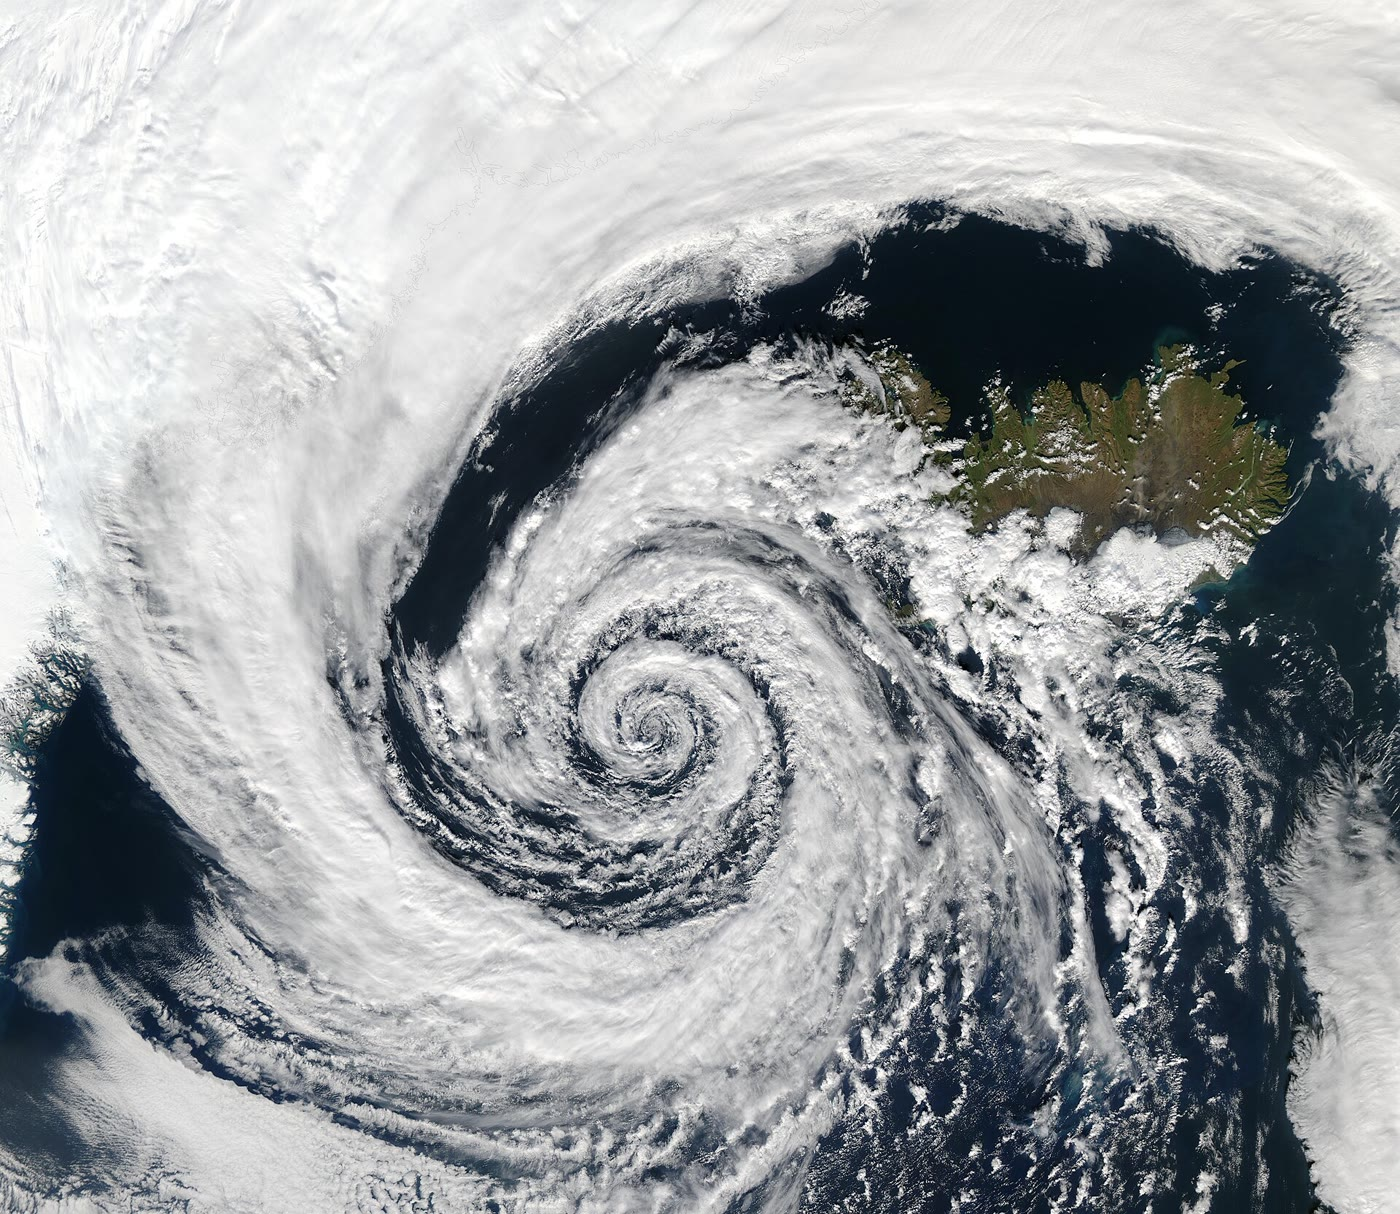
\includegraphics[width=0.58\linewidth]{images/book4/b2-22-iceland-low.jpg}
\par\smallskip{\small Uma baixa profunda ao largo da costa sudoeste da Islândia, 4 de setembro de 2003, vista pelo
instrumento MODIS do satélite Aqua da NASA: as faixas de nuvens espiralam para o centro. (NASA
Goddard Space Flight Center, MODIS Rapid Response Team, Jacques Descloitres, domínio público, via
Wikimedia Commons.)}
\end{omfigure}

\section{Correntes de jato e ondas de Rossby}\label{sec:b2:weather-systems:rossby}

Os ciclones não estão espalhados ao acaso. O jato polar, o núcleo rápido dos ventos de oeste acima da
frente polar, acompanha a posição e o movimento das altas e baixas das latitudes
médias; é mais rápido ao longo de seus núcleos de jato (jet streaks), os trechos onde sua velocidade é máxima, e
não circunda o polo como um anel: ele serpenteia.
% ledger: nws4:polar-front, nws4:jet-streak

\begin{definition}[Onda de Rossby; cavado e crista em altitude]\label{def:b2:weather-systems:rossby}
Uma \emph{onda de Rossby}\index{onda de Rossby} é uma onda do escoamento de oeste da alta troposfera,
uma série de cavados e cristas de milhares de quilômetros de comprimento, com grande amplitude norte--sul.
Um \emph{cavado em altitude}\index{cavado em altitude} é uma região alongada de pressão relativamente
baixa numa tal onda, onde o escoamento se curva em direção ao equador; uma \emph{crista em
altitude}\index{crista em altitude} é uma região alongada de pressão relativamente alta, onde ele
se curva em direção ao polo.
\end{definition}
% ledger: nws4:rossby

As \omterm{def:b2:weather-systems:rossby}{ondas de Rossby} existem porque o parâmetro de Coriolis cresce em direção ao polo. O ar empurrado para o polo
encontra um $f$ maior e, conservando sua vorticidade absoluta, volta em direção ao equador; o ar
empurrado para o equador volta em direção ao polo. A taxa com que $f$ cresce para o norte,
$\beta = \mathrm{d}f/\mathrm{d}y = 2\Omega\cos\varphi/a$, sendo $a$ o raio da Terra, fixa
sua velocidade. O volume do terceiro ano deduz, da conservação da vorticidade, a velocidade de fase de uma
onda de comprimento de onda $\lambda$ num vento de oeste uniforme $U$:
\[
  c = U - \frac{\beta}{k^2}, \qquad k = \frac{2\pi}{\lambda} .
\]
Admita-se aqui. Em relação ao ar, toda \omterm{def:b2:weather-systems:rossby}{onda de Rossby} se move para oeste, e tanto mais depressa
quanto mais longa; o vento a leva para leste. As ondas curtas são levadas para leste quase à velocidade do vento,
as longas derivam lentamente, ficam paradas ou até se movem para oeste.
% ledger: earth:Trot, earth:Rmean

\begin{example}[Três ondas a 45° N]\label{ex:b2:weather-systems:rossby}
Com $\Omega = \qty{7.292e-5}{s^{-1}}$ (um dia sideral de \qty{23.9345}{h}) e $a =
\qty{6371}{km}$, $\beta = \qty{1.62e-11}{m^{-1}.s^{-1}}$ a \ang{45} N. Num vento de oeste de
\qty{15}{m/s}, uma onda de \qty{4000}{km} tem $\beta/k^2 = \qty{6.6}{m/s}$ e move-se para leste a
\qty{8.4}{m/s}; uma de \qty{6000}{km} tem $\beta/k^2 = \qty{14.8}{m/s}$ e quase não se move,
\qty{0.2}{m/s}; uma de \qty{8000}{km} move-se para oeste a \qty{11.2}{m/s}.
\end{example}
% ledger: earth:Trot, earth:Rmean

Os cavados das ondas longas movem-se lentamente e duram muito; as ondas curtas que viajam através
deles, os cavados de onda curta, induzem ar ascendente à sua frente, do seu lado leste, onde a
pressão à superfície cai e as baixas se desenvolvem. Um cavado cujo eixo se inclina de sudeste para noroeste
é muitas vezes sinal de um sistema que se desenvolve ou se intensifica.
% ledger: nws4:rossby

\begin{omfigure}
\centering
\begin{tikzpicture}[font=\scriptsize, >=Stealth]
\foreach \lat/\pa in {30/-72, 45/-72, 60/-108} {
  \pgfmathsetmacro{\r}{6.0*tan((90-\lat)/2)}
  \draw[black!25] (0,0) circle (\r);
  \node[black!50, fill=white, inner sep=1pt] at (\pa:\r) {\ang{\lat} N};
}
\fill (0,0) circle (0.6mm);
\node[anchor=north, black!60] at (0,-0.08) {Polo Norte};
\draw[ocBlue, very thick, smooth, samples=241, domain=0:360]
  plot ({6.0*tan((90-(47+11*cos(5*\x)))/2)*cos(\x)}, {6.0*tan((90-(47+11*cos(5*\x)))/2)*sin(\x)});
\foreach \a in {18, 90, 162, 234, 306} {
  \pgfmathsetmacro{\ra}{6.0*tan((90-(47+11*cos(5*\a)))/2)}
  \pgfmathsetmacro{\rb}{6.0*tan((90-(47+11*cos(5*(\a+2))))/2)}
  \draw[ocBlue, very thick, -{Stealth[length=2.6mm]}] (\a:\ra) -- (\a+2:\rb);
}
\pgfmathsetmacro{\rt}{6.0*tan((90-36)/2)}
\node[anchor=216, ocRed!80!black, inner sep=2pt] at (36:\rt) {cavado};
\node[anchor=0, ocRed!80!black, inner sep=2pt] at (180:\rt) {cavado};
\pgfmathsetmacro{\rr}{6.0*tan((90-58)/2)}
\node[anchor=72, ocRed!80!black, inner sep=3pt] at (72:\rr) {crista};
\end{tikzpicture}
\par\smallskip{\small \omterm{def:b2:weather-systems:rossby}{Ondas de Rossby} na corrente de jato vistas de cima do Polo Norte (esquemático):
cinco ondas em volta do hemisfério, os cavados avançando em direção ao equador e as cristas em direção ao
polo. O jato corre para leste, no sentido anti-horário visto de cima do polo (setas). Círculos de latitude
desenhados como numa carta estereográfica polar.}
\end{omfigure}
% ledger: nws4:rossby

Às vezes o padrão deixa totalmente de se mover.

\begin{definition}[Bloqueio atmosférico]\label{def:b2:weather-systems:blocking}
O \emph{bloqueio atmosférico}\index{bloqueio atmosférico} é um sistema de alta pressão grande, persistente e quase
estacionário, às vezes acompanhado de uma baixa, que interrompe o escoamento normal para leste
da corrente de jato. Os métodos de detecção de bloqueios exigem quase todos que ele dure pelo menos cinco
dias.
\end{definition}
% ledger: wang26:blocking

Um bloqueio desvia o jato e os ciclones à sua volta e mantém o mesmo tempo sobre a mesma
região durante dias: os bloqueios trazem ondas de calor, secas, incêndios florestais, vagas de frio e inundações às
latitudes médias. No fim de junho e início de julho de 2021 um forte bloqueio levou à onda de calor do
Noroeste Pacífico da América do Norte, que causou mais de mil mortes. Os processos
físicos por trás do bloqueio ainda não são bem compreendidos, e os modelos numéricos têm dificuldade em
reproduzir com que frequência os bloqueios ocorrem e quanto tempo duram.
% ledger: wang26:blocking, wang26:gaps

\section{Ciclones tropicais}\label{sec:b2:weather-systems:tropical}

Os ciclones tropicais não têm frentes nem contraste de temperatura de que se alimentar. Tiram sua energia
do oceano quente, através do calor latente da água que evaporam, tal como o \cref{ch:b2:atmospheric-thermodynamics}
o mediu. Seis condições favorecem sua formação: água do oceano a pelo menos \qty{26.5}{\celsius}
numa profundidade da ordem de \qty{50}{m}; uma atmosfera que esfria depressa o bastante com a altitude para
ser instável para a convecção úmida; uma troposfera média úmida, por volta de \qty{5}{km}; uma distância de
pelo menos cerca de \qty{500}{km} do equador, para que a força de Coriolis possa manter a baixa em
equilíbrio; uma perturbação preexistente perto da superfície; e um cisalhamento vertical do vento fraco, abaixo de cerca de
\qty{10}{m/s} entre a superfície e a alta troposfera. São necessárias, mas não
suficientes: muitas perturbações que as satisfazem nunca se desenvolvem.
% ledger: aoml:tc-genesis

Uma vez formado, um ciclone tropical é uma máquina térmica. O ar espirala para dentro sobre o mar a uma temperatura
quase constante, ganhando calor e umidade do oceano; na parede do olho sobe
adiabaticamente; no escoamento de saída perto da tropopausa perde calor por radiação a uma temperatura baixa,
quase constante; e volta a descer longe do centro, completando um ciclo que
lembra o de Carnot. O trabalho do ciclo move os ventos contra o atrito da superfície
do mar.
% ledger: gilford21:pi

\begin{omfigure}
\centering
\begin{tikzpicture}[font=\scriptsize, >=Stealth, x=1cm, y=1cm]
% sea and axis
\fill[ocBlue!12] (0,-0.35) rectangle (12.5,0);
\draw[thick, ocBlue!70!black] (0,0) -- (12.5,0);
\node[anchor=north west, ocBlue!70!black] at (8.6,-0.02) {mar quente, $T_s$};
\draw[dashed, black!50] (0,-0.35) -- (0,4.9);
\node[anchor=south, black!60] at (0,4.9) {centro};
% eyewall cloud and outflow cloud
\fill[black!14, draw=black!40] (0.9,0.25) .. controls (0.7,1.8) and (0.75,3.3) .. (0.95,4.2)
  .. controls (3.5,4.55) and (7.0,4.45) .. (9.5,4.2) .. controls (7.0,3.9) and (3.6,3.85)
  .. (2.1,3.7) .. controls (1.95,2.6) and (1.9,1.4) .. (2.0,0.25) -- cycle;
\node[black!60] at (0.45,2.0) [rotate=90] {olho};
\draw[black!50] (1.9,1.1) -- (2.45,1.1) node[anchor=west, black!70] {nuvem da parede do olho};
% the cycle
\draw[->, very thick, ocRed] (11.4,0.3) -- (2.3,0.3);
\draw[->, very thick, ocRed] (1.45,0.45) .. controls (1.4,1.6) and (1.45,3.0) .. (1.75,4.0);
\draw[->, very thick, ocBlue] (2.2,4.25) -- (11.2,4.25);
\draw[->, very thick, ocBlue] (11.6,4.05) .. controls (11.75,2.8) and (11.75,1.5) .. (11.6,0.45);
\fill (11.6,0.3) circle (0.7mm) node[right=2pt] {A};
\fill (1.45,0.3) circle (0.7mm) node[left=2pt] {B};
\fill (1.8,4.25) circle (0.7mm) node[above left=1pt] {C};
\fill (11.6,4.25) circle (0.7mm) node[above right=1pt] {D};
\node[anchor=south, align=center] at (6.5,0.35) {A$\to$B: entrada sobre o mar a cerca de $T_s$,
  recebendo calor e umidade};
\node[anchor=west, align=left] at (2.25,2.3) {B$\to$C: sobe na parede do olho,\\sem
  trocar calor (adiabática úmida)};
\node[anchor=south, align=center] at (6.5,4.62) {C$\to$D: saída perto da tropopausa a cerca de
  $T_o$, perdendo calor por radiação};
\node[anchor=east, align=right] at (11.45,2.3) {D$\to$A: desce longe\\do centro};
\end{tikzpicture}
\par\smallskip{\small A máquina térmica de um ciclone tropical, um corte vertical do centro
para fora (esquemático, fora de escala): o calor é recebido à temperatura da superfície do mar
(A$\to$B) e cedido à temperatura muito mais baixa do escoamento de saída (C$\to$D), como num ciclo
de Carnot.}
\end{omfigure}
% ledger: gilford21:pi

\begin{proposition}[Intensidade potencial]\label{prop:b2:weather-systems:pi}
\index{intensidade potencial}
A \emph{\omterm{prop:b2:weather-systems:pi}{intensidade potencial}} de um ciclone tropical, a velocidade máxima do vento perto da superfície que
o oceano e a atmosfera à sua volta conseguem sustentar, é dada aproximadamente por
\[
  V_{\max}^2 = \frac{C_k}{C_D}\,\frac{T_s - T_o}{T_o}\,\bigl(h_o^* - h^*\bigr),
\]
onde $T_s$ é a temperatura da superfície do mar, $T_o$ a temperatura do escoamento de saída, $C_k/C_D$
a razão dos coeficientes de troca de entalpia e de quantidade de movimento entre o mar e o ar,
em geral tomada igual a 0.9, e $h_o^* - h^*$ o excesso de $c_pT + gz + Lq$ na saturação à superfície
do mar sobre seu valor de saturação no ar acima da camada limite (admitido).
\end{proposition}
% ledger: gilford21:pi

A fração $(T_s - T_o)/T_o$ não é o rendimento de Carnot $(T_s - T_o)/T_s$ dos livros de
física: é maior pelo fator $T_s/T_o$, porque o atrito que dissipa o trabalho aquece
o ar que entra perto da superfície do mar, e esse calor é reutilizado pela máquina. O último
fator é o combustível. Numa atmosfera tropical cuja temperatura segue a \omterm{def:b2:atmospheric-thermodynamics:moist-adiabat}{adiabática úmida} do ar de sua
camada limite, $h^*$ é o valor de $c_pT + gz + Lq$ nesse ar, e $h_o^* - h^*$
mede quanto o ar sobre o mar está longe da saturação à temperatura do mar:
\[
  h_o^* - h^* \approx c_p\,(T_s - T_a) + L\,(q_s^* - q_a),
\]
sendo $T_a$ e $q_a$ a temperatura e a \omterm{def:b2:atmospheric-thermodynamics:moist-air}{umidade específica} do ar perto da superfície e
$q_s^*$ a \omterm{def:b2:atmospheric-thermodynamics:moist-air}{umidade específica} de saturação à temperatura da superfície do mar.
% ledger: gilford21:pi

\begin{example}[Uma intensidade potencial]\label{ex:b2:weather-systems:pi}
Sobre um mar a \qty{29}{\celsius} o ar a \qty{1015}{hPa} está a \qty{28}{\celsius} com uma
umidade relativa de \qty{80}{\percent}, e o escoamento de saída está a \qty{200}{K}, uma média anual
típica sobre os oceanos tropicais quentes. Pelas \cref{prop:b2:atmospheric-thermodynamics:es,prop:b2:atmospheric-thermodynamics:humidity},
$e_s(\qty{29}{\celsius}) = \qty{41.0}{hPa}$, logo $q_s^* = \qty{25.5}{g/kg}$, e o ar, com
$e = 0.8 \times \qty{38.7}{hPa}$, tem $q_a = \qty{19.2}{g/kg}$. Então $h_o^* - h^* = 1004.5 \times
1 + 2.501 \times 10^6 \times 0.0063 = \qty{16.8}{kJ/kg}$, o fator $(T_s - T_o)/T_o$ é
$(302.15 - 200)/200 = 0.511$, e $V_{\max} = \sqrt{0.9 \times 0.511 \times 16\,800} =
\qty{88}{m/s}$.
\end{example}
% ledger: gilford21:pi

As tempestades mais fortes chegam perto desses valores: o topo da escala de Saffir--Simpson, a categoria
5, começa em \qty{70}{m/s}, e cinco tempestades recentes ultrapassaram \qty{86}{m/s}. A maioria das tempestades
raramente atinge sua \omterm{prop:b2:weather-systems:pi}{intensidade potencial}: as tempestades reais raramente estão no estado estacionário que a teoria
supõe, e a teoria deixa de fora o cisalhamento vertical do vento, o ar seco aspirado para a tempestade e a
subsidência do ar à sua volta, que enfraquecem uma tempestade.
% ledger: wk24:scale, gilford21:limits, aoml:tc-weaken

\begin{omfigure}
\centering
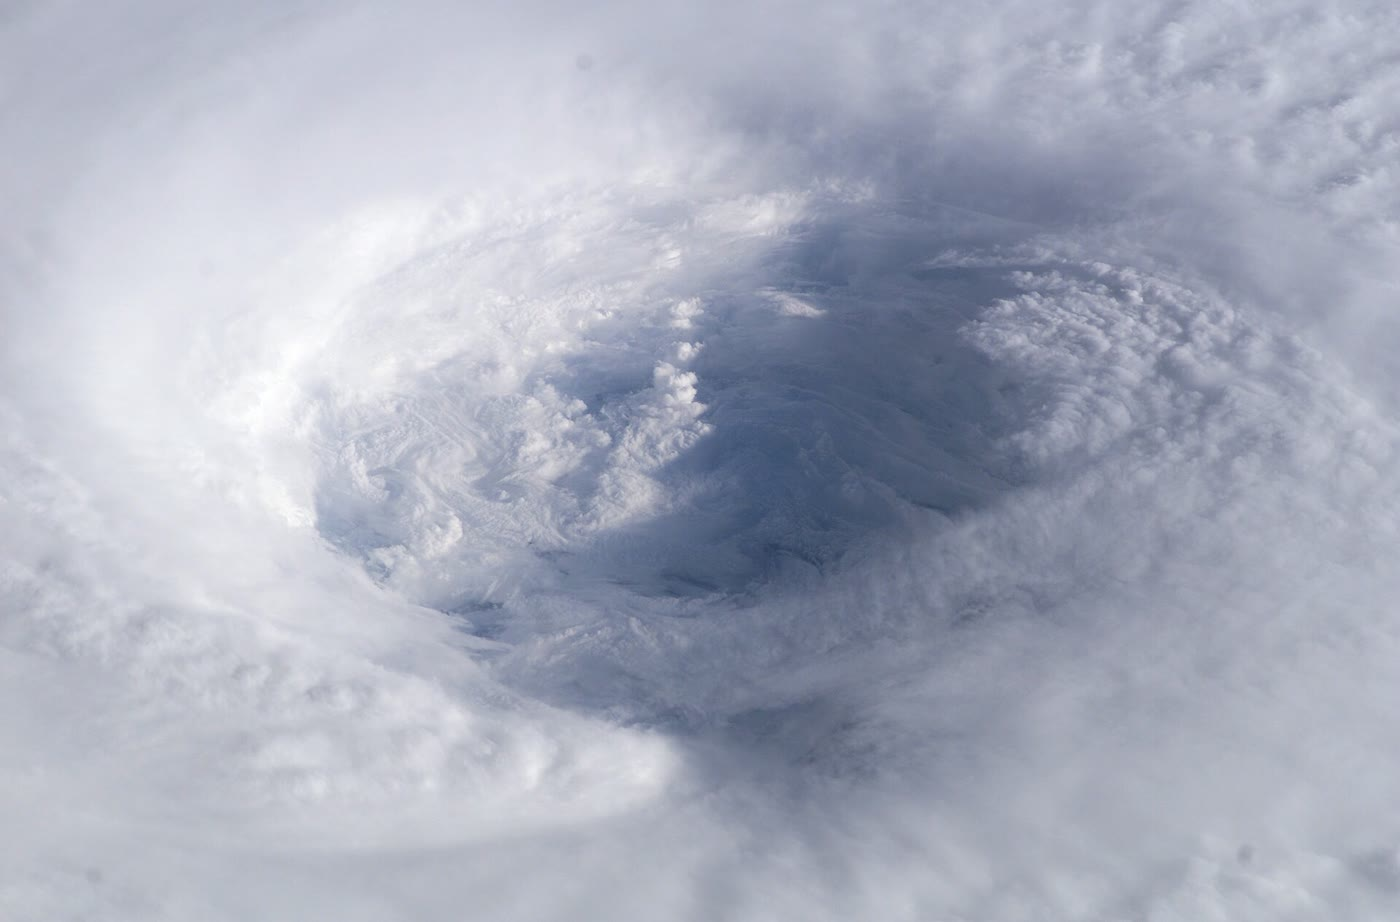
\includegraphics[width=0.62\linewidth]{images/book4/b2-22-isabel-eye.jpg}
\par\smallskip{\small O olho do furacão Isabel, 13 de setembro de 2003, fotografado da
Estação Espacial Internacional: a parede do olho desce como um estádio até as nuvens baixas do olho.
(Astronauta da NASA Ed Lu, domínio público, via Wikimedia Commons.)}
\end{omfigure}

\section{Previsão numérica do tempo}\label{sec:b2:weather-systems:nwp}

\begin{definition}[Previsão numérica do tempo; assimilação de dados; previsão por conjunto; limite de previsibilidade]\label{def:b2:weather-systems:nwp}
A \emph{previsão numérica do tempo}\index{previsão numérica do tempo} é a previsão por
computador: as equações que governam o movimento, a energia e a água da atmosfera são
integradas para a frente no tempo a partir de seu estado observado. A \emph{assimilação de dados}\index{assimilação de dados}
combina as observações mais recentes com uma previsão de curto prazo feita a partir de observações
anteriores para obter a melhor estimativa do estado presente, a análise, da qual parte a
previsão. Uma \emph{previsão por conjunto}\index{previsão por conjunto} é um conjunto de previsões rodadas
a partir de estados iniciais ligeiramente diferentes, e com versões ligeiramente diferentes do modelo, para
mostrar a gama de tempos possíveis e sua probabilidade. O \emph{limite de
previsibilidade}\index{limite de previsibilidade} é o prazo além do qual uma previsão do estado do
tempo não é melhor que um palpite baseado no clima, porque os erros do estado inicial
cresceram até ficarem tão grandes quanto as diferenças entre dois estados quaisquer da atmosfera.
\end{definition}
% ledger: nws4:nwp, ecmwf4:da, ecmwf4:ens-fs, krish19:predictability

A primeira previsão numérica foi calculada em 1950 no ENIAC, um dos primeiros computadores
eletrônicos. Um modelo global divide hoje a atmosfera numa grade de células de alguns quilômetros
de lado e parte de uma análise que combina observações de estações meteorológicas, aviões,
radiossondas, navios, boias e, sobretudo, satélites, que dão a maior contribuição para a
qualidade das previsões globais. Num grande centro de previsão o conjunto
tem 51 membros, uma rodada de controle e 50 perturbadas, com uma resolução de cerca de \qty{9}{km}, rodado
duas vezes por dia até 15 dias à frente.
% ledger: krish19:predictability, ecmwf4:da, ecmwf4:ens

Por que perturbar uma previsão que poderia partir da melhor análise? Porque a atmosfera é
caótica, sensível a seu estado inicial. Um sistema de três variáveis, publicado em 1963, mostra-o
na menor escala.

\begin{proposition}[O sistema de Lorenz]\label{prop:b2:weather-systems:lorenz}
O sistema
\[
  \dot x = \sigma(y - x), \qquad \dot y = x(r - z) - y, \qquad \dot z = xy - bz,
\]
com $\sigma = 10$, $r = 28$ e $b = 8/3$, tem as seguintes propriedades.
\begin{enumerate}
  \item Seus pontos fixos são a origem e $C_\pm = \bigl(\pm\sqrt{b(r - 1)}, \pm\sqrt{b(r - 1)},
        r - 1\bigr) = (\pm 8.49, \pm 8.49, 27)$.
  \item Todo volume em seu espaço de fases encolhe como $\mathrm{e}^{-(\sigma + 1 + b)t}$: suas
        trajetórias terminam num conjunto de volume nulo, o atrator.
  \item No atrator, duas trajetórias que partem a uma pequena distância $\delta_0$ uma da outra separam-se,
        em média, como $\delta(t) \approx \delta_0\,\mathrm{e}^{\lambda t}$, com $\lambda =
        0.906$, até $\delta$ atingir o tamanho do atrator (calculado, admitido). Os pequenos
        erros duplicam a cada $\ln 2/\lambda = 0.77$ unidades de tempo.
\end{enumerate}
\end{proposition}
% ledger: nolitia22:lorenz

\begin{proof}[Demonstração de 1 e 2]
Num ponto fixo, $y = x$ pela primeira equação; a terceira dá $z = x^2/b$; a segunda
torna-se $x(r - 1 - x^2/b) = 0$, logo $x = 0$ ou $x^2 = b(r - 1) = 72$. A divergência do
campo vetorial é $\partial_x\dot x + \partial_y\dot y + \partial_z\dot z = -\sigma - 1 - b$, uma
constante, e pelo teorema da divergência um volume $V$ transportado pelo escoamento obedece a $\dot V =
-(\sigma + 1 + b)V$.
\end{proof}

As figuras mostram o que a proposição significa. Duas rodadas que partem a \num{e-5} uma da outra seguem-se
durante umas quinze unidades de tempo, depois separam-se de vez: cada uma ainda parece uma
trajetória plausível do sistema, mas já não são a mesma trajetória. Em média sobre 200 pares de
rodadas iniciadas a \num{e-8} uma da outra, a distância cresce exponencialmente à taxa $\lambda$, uma
reta em escala logarítmica, até saturar no tamanho do atrator. Qualquer que seja o
erro inicial, ele atinge esse tamanho: um erro inicial menor apenas adia o momento, em
$\ln 10/\lambda = 2.5$ unidades de tempo para cada redução por dez.
% ledger: nolitia22:lorenz

\begin{omfigure}
\centering
% figdata/bachelor-2/weather.py parts traj, butterfly
\begin{tikzpicture}
\begin{groupplot}[group style={group size=2 by 1, horizontal sep=1.5cm},
  tick label style={font=\scriptsize}, label style={font=\small}]
\nextgroupplot[width=0.58\linewidth, height=5.0cm, xmin=0, xmax=30, ymin=-22, ymax=22,
  xlabel={tempo}, ylabel={$x$}, legend style={font=\scriptsize, at={(0.5,1.02)},
  anchor=south, draw=none, legend columns=2, /tikz/every even column/.append style={column
  sep=0.4cm}}, legend cell align=left]
\addplot[ocBlue, thin] table[x=t, y=x1] {figdata/out/bachelor-2-weather-traj.dat};
\addlegendentry{rodada 1}
\addplot[ocRed, thin, densely dashed] table[x=t, y=x2] {figdata/out/bachelor-2-weather-traj.dat};
\addlegendentry{rodada 2, iniciada a \num{e-5}}
\nextgroupplot[width=0.4\linewidth, height=5.0cm, xmin=-22, xmax=22, ymin=0, ymax=52,
  xlabel={$x$}, ylabel={$z$}]
\addplot[black!70, very thin] table[x=x, y=z] {figdata/out/bachelor-2-weather-butterfly.dat};
\addplot[only marks, mark=*, mark size=1.3pt, ocRed] coordinates {(8.485,27) (-8.485,27)};
\end{groupplot}
\end{tikzpicture}
\par\smallskip{\small O sistema de Lorenz ($\sigma = 10$, $r = 28$, $b = 8/3$), integrado pelo
método de Runge--Kutta com um passo de tempo de 0.01. Esquerda: duas rodadas que partem a \num{e-5} uma da outra em $x$
no atrator. Direita: uma rodada ao longo de 40 unidades de tempo, vista ao longo de $y$, com os pontos fixos
$C_\pm$ (vermelho).}
\end{omfigure}
% ledger: nolitia22:lorenz

\begin{omfigure}
\centering
% figdata/bachelor-2/weather.py part growth
\begin{tikzpicture}
\begin{axis}[width=0.72\linewidth, height=5.6cm, xmin=0, xmax=30, ymode=log, ymin=1e-9,
  ymax=1e3, ytick={1e-9,1e-7,1e-5,1e-3,1e-1,1e1,1e3}, xlabel={tempo}, ylabel={distância entre as rodadas}, tick label style={font=\scriptsize},
  label style={font=\small}, legend style={font=\scriptsize, at={(0.02,0.98)}, anchor=north west,
  draw=none, fill=none}, legend cell align=left, unbounded coords=discard, grid=major,
  grid style={black!8}]
\addplot[ocBlue, line width=1.6pt, opacity=0.55] table[x=t, y expr=10^\thisrow{log10d}]
  {figdata/out/bachelor-2-weather-growth.dat};
\addlegendentry{média de 200 pares (geométrica)}
\addplot[black, densely dashed, thin] table[x=t, y expr=10^\thisrow{fit}]
  {figdata/out/bachelor-2-weather-growth.dat};
\addlegendentry{exponencial ajustada, $t = 2$ a 16}
\end{axis}
\end{tikzpicture}
\par\smallskip{\small Crescimento da distância entre pares de rodadas do sistema de Lorenz iniciadas
a \num{e-8} uma da outra. A reta ajustada sobe um fator dez a cada 2.57 unidades de tempo, uma taxa de 0.897;
o maior expoente de Lyapunov, calculado renormalizando um único par ao longo de 2000 unidades de tempo, é
0.909, contra 0.906 publicado. O crescimento para no tamanho do atrator.}
\end{omfigure}
% ledger: nolitia22:lorenz

A atmosfera comporta-se da mesma maneira, com muito mais variáveis e com erros que crescem a
taxas diferentes em escalas diferentes. A partir das previsões dos anos 1980, verificou-se que os pequenos erros
duplicavam em cerca de 2.4 dias, e a previsão confiável do estado do tempo para antes de
cerca de dez dias. Experimentos que reduzem a incerteza atual do estado inicial, com um modelo
suposto perfeito, concluem que condições iniciais perfeitas acrescentariam apenas quatro a cinco dias, e
que uma redução de 90 por cento já dá quase tudo: à medida que os erros ficam menores, crescem
mais depressa, através da liberação de calor latente na convecção, em escalas menores do que a previsão
consegue resolver. O \omterm{def:b2:weather-systems:nwp}{limite de previsibilidade} das latitudes médias fica por volta de duas semanas. As previsões
ganham cerca de um dia por década porque observações, assimilação e modelos melhores as aproximam
desse limite; elas não podem ultrapassá-lo.
% ledger: krish19:predictability, selz22:limit, bauer:day-per-decade

O conjunto transforma isso numa ferramenta. Seus membros partem de análises que diferem mais ou menos
tanto quanto a própria análise é incerta; enquanto concordam, a previsão é precisa; quando se
dispersam, a previsão tem de dizê-lo, e dá probabilidades. Uma previsão diz-se confiável quando
os eventos que anuncia com uma probabilidade de \qty{70}{\percent} acontecem em \qty{70}{\percent} dos
casos.
% ledger: ecmwf4:ens-fs

\begin{inthelab}[Um dia num centro de previsão]
\begin{minipage}[t]{0.54\linewidth}\vspace{0pt}
Num centro de previsão global o dia gira em torno de dois horários, 00 e 12 UTC. As observações válidas
por volta de cada horário chegam aos milhões, de satélites, radiossondas, aviões, navios e
boias e estações meteorológicas; a \omterm{def:b2:weather-systems:nwp}{assimilação de dados} combina-as com a previsão curta anterior para
obter a análise. Os modelos partem dela, o conjunto também, e as previsões chegam a seus usuários
várias horas depois, após os supercomputadores terem rodado os 15 dias à frente. Os previsores então
comparam as rodadas, conferem-nas com as observações mais recentes e as imagens de satélite, acompanham
os ciclones e as frentes, e transformam as probabilidades do conjunto em avisos e
previsões.
\end{minipage}\hfill
\begin{minipage}[t]{0.42\linewidth}\vspace{0pt}
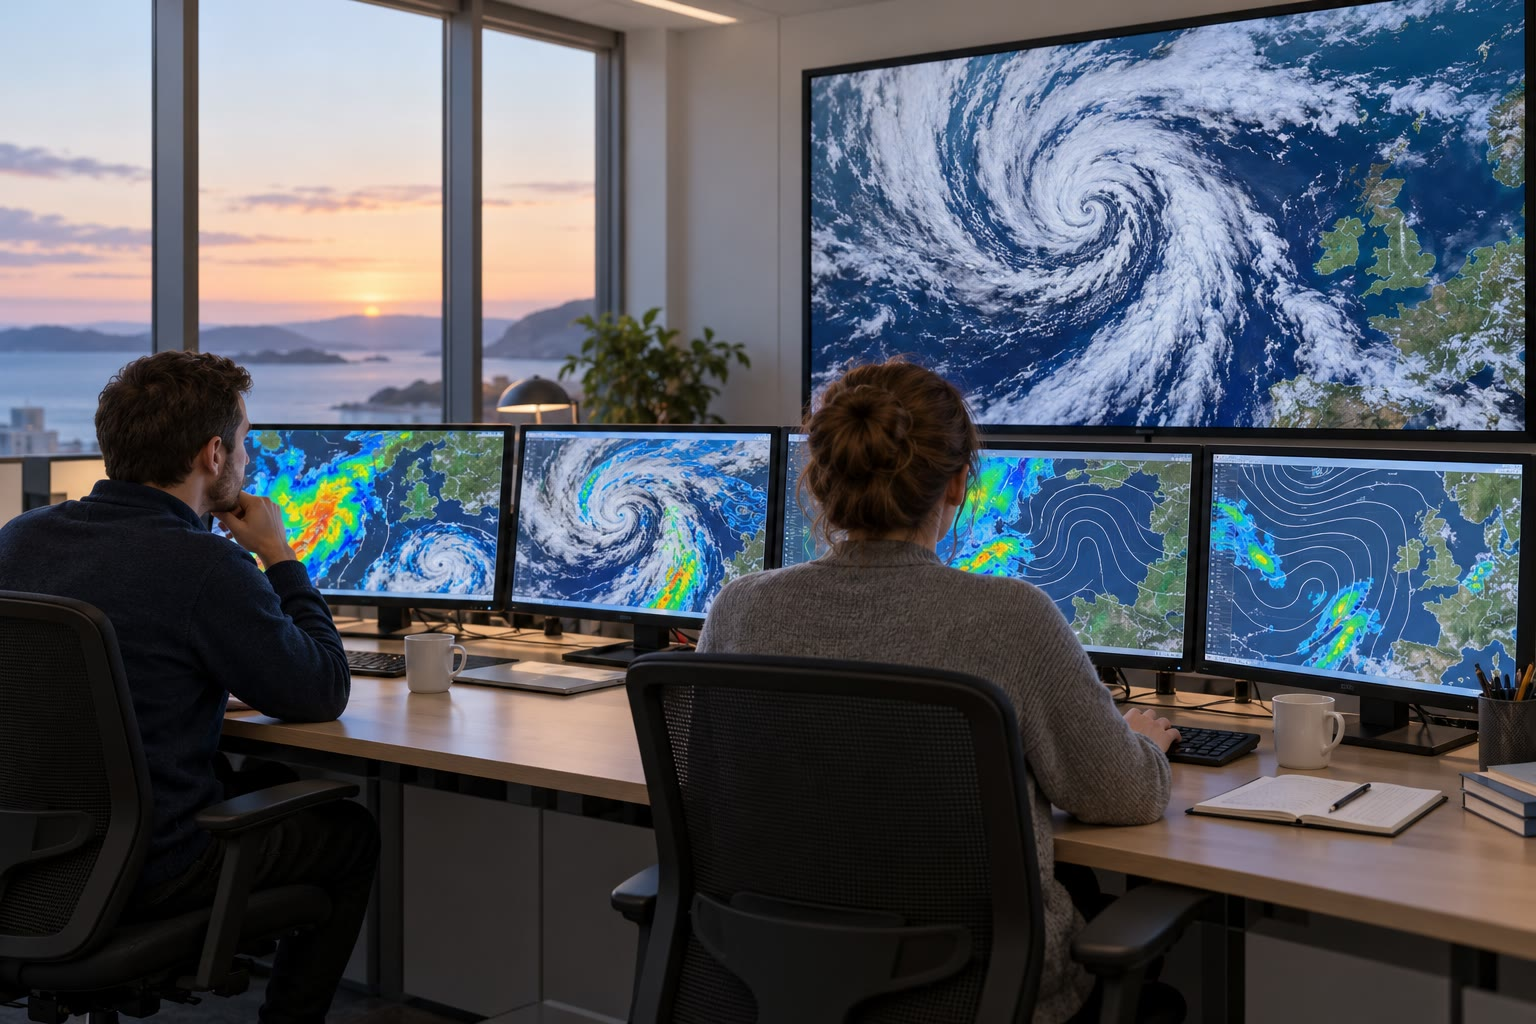
\includegraphics[width=\linewidth]{images/book4/ai/b2-forecast-office.jpg}

{\scriptsize Previsores trabalhando diante de imagens de satélite e cartas de modelos
(ilustração gerada por IA).}
\end{minipage}
% ledger: ecmwf4:ens, ecmwf4:da, mo:how-forecasts
\end{inthelab}

\section*{Exercícios}\label{sec:b2:weather-systems:exercises}

Dados para os exercícios, salvo indicação em contrário: $\Omega = \qty{7.292e-5}{s^{-1}}$, $a =
\qty{6371}{km}$, $g = \qty{9.81}{m.s^{-2}}$, $c_p = \qty{1004.5}{J.kg^{-1}.K^{-1}}$, $L =
\qty{2.501e6}{J/kg}$, e a \omterm{def:b2:atmospheric-thermodynamics:moist-air}{pressão de vapor} de saturação dos exercícios do
\cref{ch:b2:atmospheric-thermodynamics}.
% ledger: earth:Trot, earth:Rmean

\begin{exercise}[$\star$]\label{exo:b2:weather-systems:1}
A \ang{50} N uma frente fria separa um ar a \qty{275}{K} de um ar a \qty{281}{K}, e o vento
ao longo dela varia \qty{15}{m/s}. (a) Calcule $f$. (b) Calcule a inclinação da \omterm{def:b2:weather-systems:fronts}{superfície frontal},
na forma 1 para $N$. (c) A que distância atrás da frente no solo a \omterm{def:b2:weather-systems:fronts}{superfície frontal} atinge
\qty{1}{km}? (d) O que acontece com a inclinação se o contraste de temperatura dobrar, com a mesma mudança
de vento?
\end{exercise}

\begin{exercise}[$\star$]\label{exo:b2:weather-systems:2}
Uma \omterm{def:b2:weather-systems:fronts}{superfície frontal} quente sobe a 1 para 150 e move-se a \qty{25}{km/h}. (a) A que distância à frente da
frente no solo a \omterm{def:b2:weather-systems:fronts}{superfície frontal} está a \qty{6}{km} de altura? (b) Um observador vê nuvens altas se formarem
sobre ela ali. Quanto tempo depois a frente chega ao observador? (c) Descreva a sequência de
nuvens que o observador vê nesse intervalo.
\end{exercise}
% ledger: ucar:warm-front

\begin{exercise}[$\star$]\label{exo:b2:weather-systems:3}
Num mapa do Hemisfério Norte, (a) uma linha com triângulos azuis do seu lado sudeste estende-se para sudoeste
a partir de uma baixa; (b) uma linha com semicírculos vermelhos do seu lado norte estende-se para leste a partir da mesma baixa; (c) uma
linha roxa com os dois símbolos vai de outra baixa até um ponto onde começam duas outras frentes;
(d) uma linha alterna triângulos azuis do seu lado sul e semicírculos vermelhos do seu lado norte.
Dê o nome de cada frente, diga onde está o ar frio e para que lado cada uma se move.
\end{exercise}
% ledger: ucar4:stationary-occluded, nws4:occluded

\begin{exercise}[$\star$]\label{exo:b2:weather-systems:4}
A \ang{45} N num vento de oeste de \qty{12}{m/s}: (a) calcule $\beta$. (b) Calcule a velocidade de fase
de ondas de \qty{4000}{km} e de \qty{8000}{km}. (c) Para que lado cada uma se move, e quanto num
dia?
\end{exercise}

\begin{exercise}[$\star\star$]\label{exo:b2:weather-systems:5}
(a) Mostre que uma \omterm{def:b2:weather-systems:rossby}{onda de Rossby} fica parada num vento de oeste $U$ quando $\lambda = 2\pi\sqrt{U/\beta}$.
(b) Calcule-o a \ang{45} N para $U = \qty{12}{m/s}$. (c) Quantas dessas ondas cabem em volta do
círculo de latitude? (d) Por que um vento de oeste mais forte favoreceria ondas estacionárias menos numerosas e mais longas?
\end{exercise}

\begin{exercise}[$\star\star$]\label{exo:b2:weather-systems:6}
Para o sistema de Lorenz: (a) verifique que $C_+$ é um ponto fixo calculando as três derivadas
nele. (b) Por que fator um pequeno volume do espaço de fases encolhe numa unidade de tempo? (c) Por que
isso não impede duas trajetórias vizinhas de se separarem?
\end{exercise}

\begin{exercise}[$\star\star$]\label{exo:b2:weather-systems:7}
Tome $\lambda = 0.906$ para o sistema de Lorenz e um atrator de tamanho 10. (a) Calcule o
tempo de duplicação dos pequenos erros. (b) Quanto tempo um erro de \num{e-8} leva para atingir o tamanho do
atrator? (c) Quanto um erro inicial mil vezes menor adia esse momento? Que
fração do tempo encontrado em (b) isso representa?
\end{exercise}
% ledger: nolitia22:lorenz

\begin{exercise}[$\star\star$]\label{exo:b2:weather-systems:8}
Um mar a \qty{303}{K} tem um escoamento de saída a \qty{195}{K}; o desequilíbrio é $h_o^* - h^* =
\qty{15}{kJ/kg}$ e $C_k/C_D = 0.9$. (a) Calcule a \omterm{prop:b2:weather-systems:pi}{intensidade potencial}. (b) Compare-a com
o limiar da categoria 5 e com as tempestades recentes mais rápidas. (c) Por que a maioria das tempestades não a
atinge?
\end{exercise}
% ledger: gilford21:pi, wk24:scale

\begin{exercise}[$\star\star$]\label{exo:b2:weather-systems:9}
Para a tempestade do \cref{exo:b2:weather-systems:8}: (a) calcule o rendimento de Carnot de uma máquina
que funcione entre a superfície do mar e o escoamento de saída. (b) Calcule o fator $(T_s - T_o)/T_o$ da
\cref{prop:b2:weather-systems:pi} e a razão entre os dois. (c) Explique a diferença.
\end{exercise}
% ledger: gilford21:pi

\begin{exercise}[$\star\star\star$]\label{exo:b2:weather-systems:10}
(a) Deduza de novo a \cref{prop:b2:weather-systems:slope}, mantendo as densidades exatas, e mostre que
o ar frio deve ficar por baixo. (b) Através de uma zona frontal de \qty{50}{km} de largura a \ang{45} N o vento
ao longo da frente varia \qty{10}{m/s}. Calcule a vorticidade relativa da zona e compare-a
com $f$. (c) A zona é ciclônica ou anticiclônica?
\end{exercise}

\begin{exercise}[$\star\star\star$]\label{exo:b2:weather-systems:11}
Suponha que os erros de previsão dupliquem a cada 2.4 dias, comecem em \qty{0.5}{K} e fiquem inúteis em
\qty{6}{K}. (a) Encontre o horizonte das previsões úteis. (b) Por que fator o erro inicial deve
diminuir a cada década para ganhar um dia por década, se o modelo fosse perfeito? (c) Os experimentos concluem que
um erro inicial dez vezes menor ganha apenas 4 a 5 dias. Que tempo de duplicação isso implica para os
pequenos erros, e o que diz sobre a maneira como os pequenos erros crescem?
\end{exercise}
% ledger: krish19:predictability, selz22:limit, bauer:day-per-decade

\begin{exercise}[$\star\star\star$]\label{exo:b2:weather-systems:12}
Tome o \cref{ex:b2:weather-systems:pi} e aqueça o mar e o ar em \qty{1}{K}, mantendo a
umidade relativa e a temperatura do escoamento de saída. (a) Recalcule $q_s^*$, $q_a$ e o
desequilíbrio. (b) Recalcule a \omterm{prop:b2:weather-systems:pi}{intensidade potencial}. (c) Em quantos por cento por kelvin
ela aumenta, e que fator contribui mais?
\end{exercise}
% ledger: gilford21:pi

\begin{problem}[{Problema de fim de semana --- a que distância à frente?}]\label{pb:b2:weather-systems:1}
Uma carta do tempo inventada a \ang{50} N mostra uma frente fria avançando sobre uma cidade, com uma \omterm{def:b2:weather-systems:rossby}{onda
de Rossby} na corrente de jato acima. O problema acompanha a frente, depois a onda, e então pergunta com que
antecedência qualquer uma delas pode ser prevista. Use os dados dos exercícios.

\medskip\noindent\textbf{Parte I --- A frente.}
Às 06 UTC a frente fria está \qty{480}{km} a oeste da cidade, às 12 UTC a \qty{390}{km}. Atrás dela
o ar está a \qty{277}{K}, no setor quente a \qty{285}{K}, e o vento ao longo da frente
varia \qty{16}{m/s} através dela.
\begin{enumerate}
  \item Encontre a velocidade da frente.
  \item A que horas ela chega à cidade?
  \item Calcule $f$ a \ang{50} N.
  \item Calcule a inclinação da \omterm{def:b2:weather-systems:fronts}{superfície frontal}.
  \item A que altura está a \omterm{def:b2:weather-systems:fronts}{superfície frontal} acima da cidade seis horas depois da passagem da frente?
  \item Quanto tempo depois da passagem o ar frio atinge \qty{1.5}{km} acima da cidade?
  \item Que tempo a cidade vê quando a frente passa, e como varia a pressão?
\end{enumerate}

\medskip\noindent\textbf{Parte II --- A onda em altitude.}
No jato acima, o vento de oeste é de \qty{20}{m/s} e a onda tem um comprimento de onda de \qty{5000}{km}.
\begin{enumerate}[resume]
  \item Calcule $\beta$ a \ang{50} N.
  \item Calcule $k$ e $\beta/k^2$.
  \item Encontre a velocidade de fase da onda.
  \item Quanto um cavado se desloca em 24 horas?
  \item Encontre o comprimento de onda que ficaria parado nesse vento, e quantas dessas ondas cabem
        em volta de \ang{50} N.
  \item Onde, em relação ao \omterm{def:b2:weather-systems:rossby}{cavado em altitude}, o ciclone de superfície deveria se aprofundar?
\end{enumerate}

\medskip\noindent\textbf{Parte III --- Uma atmosfera de brinquedo.}
Na figura do crescimento dos erros no sistema de Lorenz, a reta ajustada passa por
cerca de \num{5e-7} em $t = 4$ e \num{3.9e-3} em $t = 14$.
\begin{enumerate}[resume]
  \item A partir dessas duas leituras, calcule a taxa de crescimento $\lambda$.
  \item Calcule o tempo de duplicação.
  \item Compare com o expoente publicado 0.906.
  \item Por que a distância para de crescer, por volta de 15?
  \item Quanto mais tarde um erro dez vezes menor atinge esse tamanho?
\end{enumerate}

\medskip\noindent\textbf{Parte IV --- A que distância à frente?}
Tome o tempo de duplicação de 2.4 dias encontrado para os pequenos erros das previsões dos anos 1980, um
erro inicial de \qty{0.1}{\celsius} na temperatura num certo nível, e uma previsão que fica
inútil quando o erro atinge \qty{3}{\celsius}.
\begin{enumerate}[resume]
  \item Quantas duplicações separam o erro inicial do erro inútil?
  \item Quantos dias isso leva?
  \item Quantos dias ganharia a redução do erro inicial à metade?
  \item Com a estimativa anterior de um tempo de duplicação de 5 dias, que horizonte se obteria?
  \item Os experimentos modernos concluem que um erro inicial dez vezes menor, e mesmo um estado
        inicial perfeito, ganham apenas 4 a 5 dias. Por que isso sugere que a estimativa da
        questão 20 é otimista?
  \item Em resumo: com quantos dias de antecedência esta previsão poderia ser útil?
\end{enumerate}
\end{problem}
% ledger: krish19:predictability, selz22:limit, nolitia22:lorenz, ucar:cold-front
